\chapter{Wind-optimal Routing for Formation Flight}\label{chp:3}



	\section{Wind Routing Method}\label{sec:wind_method}	
		While weather is chaotic and difficult to accurately predict over longer periods of time, short term `day-to-day' weather forecasts are generally easier to predict. Aircraft flight plans, chosen prior to takeoff account for a wide variety of both predictable and unpredictable factors. This typically includes the use of weather forecasts to avoid potentially adverse weather ....

		\subsection{Generating Static Wind Fields}\label{sec:wind_fields}
			To generate wind fields, a set of evenly spaced geographical points is first generated across the entire map. Each of these points are then assigned vectors with a random direction and a random (but bounded) magnitude. 
			...
				\begin{figure}[ht]
				\centering
					\subfigure[Low volatility]
					{
					\frame{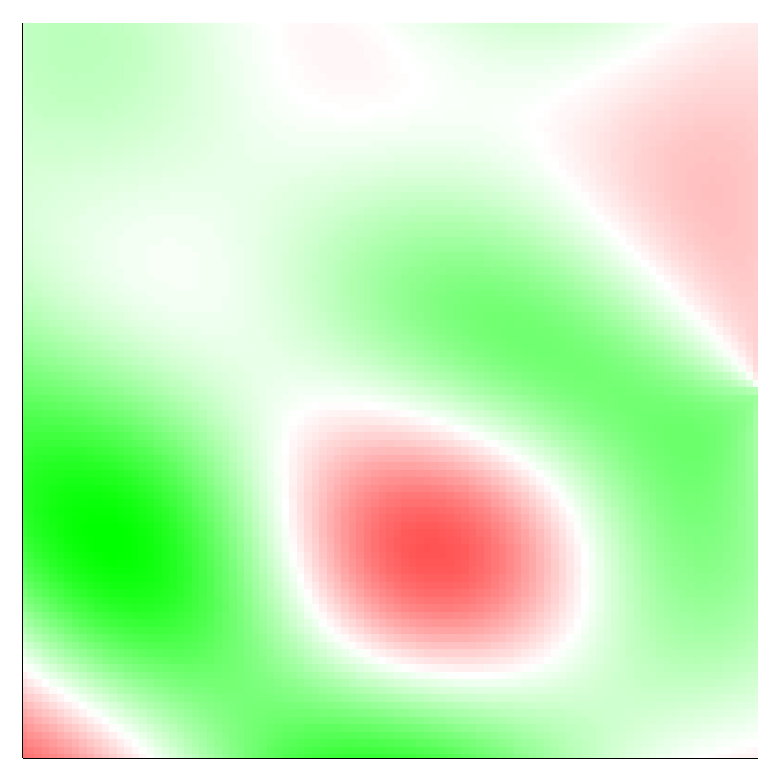
\includegraphics[width= 0.3 \columnwidth]{Chapter03/figures/Wind_plot_r1}}
					}
					\subfigure[Medium volatility]
					{
					\frame{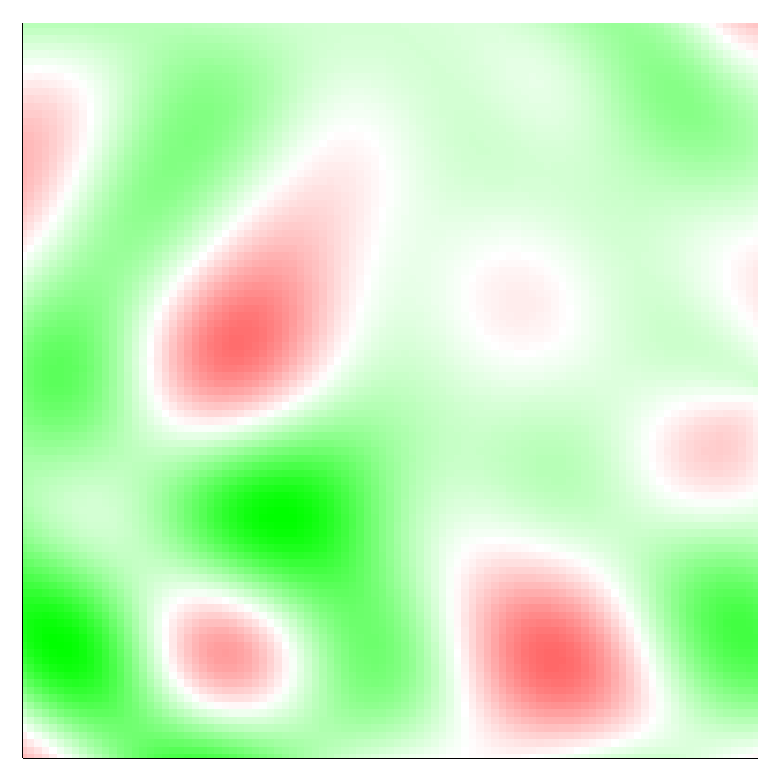
\includegraphics[width= 0.3 \columnwidth]{Chapter03/figures/Wind_plot_r2}}
					}
					\subfigure[High volatility]
					{
					\frame{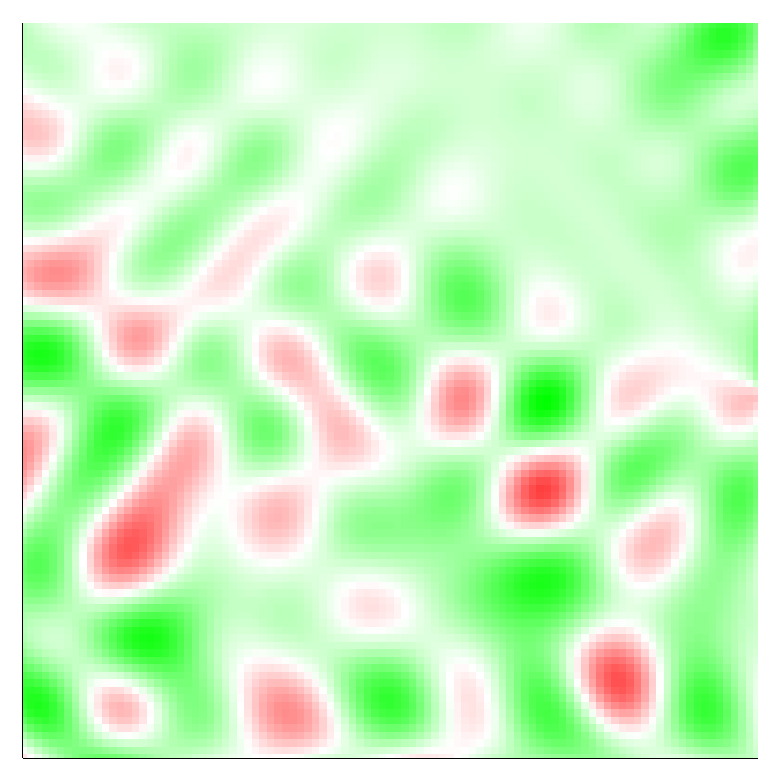
\includegraphics[width= 0.3 \columnwidth]{Chapter03/figures/Wind_plot_r4}}
					}
				\caption{Random wind fields for different levels of volatility}
					\label{fig:windfields}
				\end{figure}

		

		\input{Chapter03/Results-CS.dat}%results from casestudy variables
		\input{Chapter03/Results-CS-Est.dat}%using the Estimated Assignment method
		\input{Chapter03/Results-EAM-changes.dat}%using the Estimated Assignment method

		 \subsection{Jet-Stream West-to-East}\label{sec:WE}
		 	The formation results travelling from West-to-East over the Atlantic, with a wind field representational of the Jet-Stream, are now shown. 
		 	...

		 	results in a globally optimal solution. The resulting assignment equates to a saving of roughly \ValWindpcWE$\%$, against the corresponding solo flights routed through wind, and takes around 180 hours. This runtime break down as follows:
			\begin{samepage}
		 	\begin{description}
			 	\item[Enumeration: Solo] 210 solo flights routed for wind: 10 minutes;
			 	\item[Enumeration: Formations] 21,945 formations routed for wind: 180 hours; 
			 	\item[Assignment] MILP assignment: 4 seconds; 
			 	\item[Post-Process] None;
			 	\item[Total] 180 hours.
		 	\end{description}
		 	\end{samepage}

	 	 	A proportion of the saving achieved comes from cruising with a tailwind, so makes any possible saving clearly dependent on the particular wind field used. The routes of this solution are shown in ...

		 	If instead Method 2 is used, where the enumeration stage is done using geometric routing and then using these costs an assignment is made,  

		 	... 

		 	The resulting assignment, when routed through wind, achieves \ValGeoWindpcWE$\%$ against solo flight, but takes significantly less time at around 60 minutes. This runtime breaks down as follows: 
			\begin{samepage}
		 	\begin{description}
			 	\item[Enumeration: Formations] 21,945 formations routed geometrically: 10 seconds; 
			 	\item[Assignment] MILP assignment: 4 seconds; 
			 	\item[Post-Process: Solo] 210 solo flights routed for wind: 10 minutes.
			 	\item[Post-Process: Formations] 105 assigned formations routed for wind: 50 minutes.
			 	\item[Total] 60 minutes
		 	\end{description}
		 	\end{samepage}
		 	The geometric assignment routed through wind is plotted ... only \ValSameFormWE\ formation pairs, roughly \ValSameFormpcWE\%, remain the same between the two assignments.
		 	
		





